\newcommand{\mathsmall}[1]{\substack{\scalebox{0.8}{$#1$}}}
\begin{figure}[tbp]
\begin{tabular}{clclc}
 \begin{minipage}{0.27\textwidth}
 $\sigma:$\\
% ~ \\
 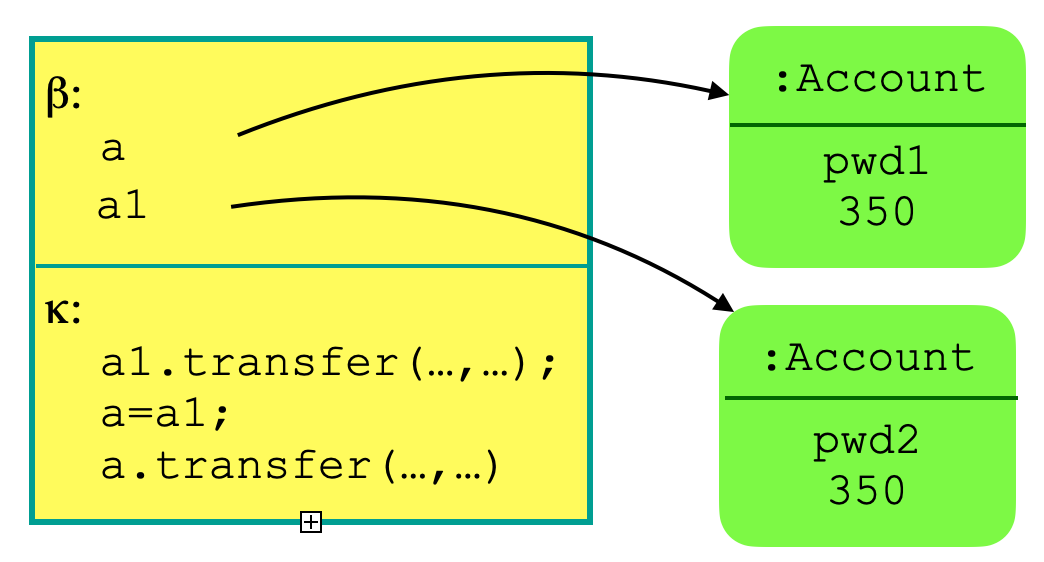
\includegraphics[width=\linewidth]{diagrams/adapt1.png}
   \end{minipage}
 & \ \ \ &
 \begin{minipage}{0.27\textwidth}
  $\sigma':$\\
 % ~ \ \\
  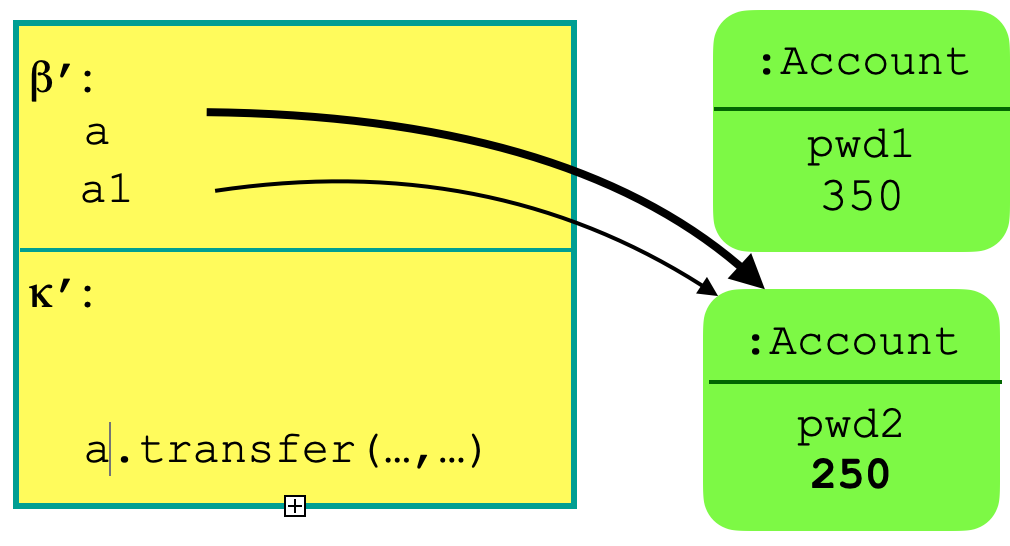
\includegraphics[width=\linewidth]{diagrams/adapt2.png}
   \end{minipage}
   & \ \ \  &
    \begin{minipage}{0.27\textwidth}
$\adapt {\sigma'}{\sigma}:$\\
% ~ \\
  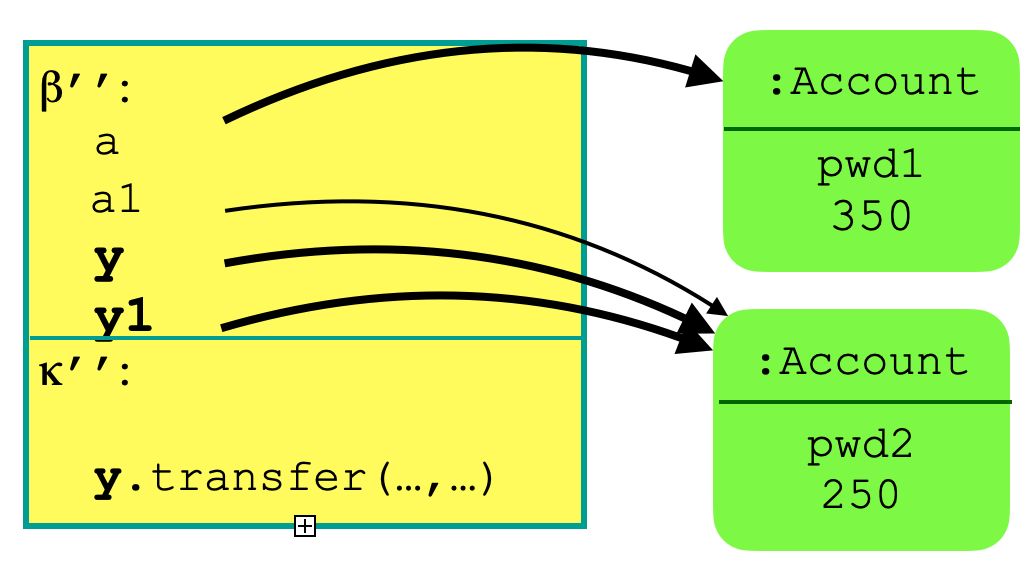
\includegraphics[width=\linewidth]{diagrams/adapt3.png}
   \end{minipage}
\end{tabular}

%\begin{tikzpicture}[->,>=to,shorten >=1pt,auto,node distance=5.5mm,
%                    thick,
%                    state/.style={circle,draw,minimum size=7mm,font=\sffamily\bfseries, color=hotpink, fill = hotpink, text = black, fill opacity = 0.5, scale=0.9},
%                    dots/.style={
%                    minimum size=7mm,
%                    font=\sffamily\Large\bfseries, 
%                    color=lightseagreen, 
%                    text = black, 
%                    fill opacity = 0.5},
%                    space/.style={
%                    minimum size=7mm,
%                    font=\sffamily\Large\bfseries, 
%                    color=lightseagreen, 
%                    text = black, 
%                    fill opacity = 0.5},
%                    arrow/.style={
%                    minimum size=7mm,
%                    font=\sffamily\Large\bfseries, 
%                    color=lightseagreen, 
%                    text = black, 
%                    fill opacity = 0.5},
%                    models/.style={
%                    minimum size=7mm,
%                    font=\sffamily\Large\bfseries, 
%                    color=lightseagreen, 
%                    text = black, 
%                    fill opacity = 0.5},
%                    decoration = snake]
%    
%    \node[space] (s) at (0,0) {};
%	\node[state, label={270:$\mathsmall{\vDash A_1}$}] (a) at (3.85,0) {$\sigma_1$};
%%	\node[space] (b) [right = of a] {};
%	\node[state, label={270:{$\mathsmall{\vDash A_2}$}}] (c) [right = of a] {$\sigma_n$};
%	\draw [decorate, ->]
%	(a) -- (c);
%\end{tikzpicture}
\caption{Illustrating adaptation
}
\label{fig:Adaptation}
\end{figure}
